\documentclass{article}
\usepackage{graphicx} % Required for inserting images
\usepackage{longtable}

\title{Assignment 3}
\author{Claire Zhang}
\date{November 11, 2023}

\begin{document}

\maketitle

\section{Balance Table}

\begin{table}[htbp]
\caption{\textbf{Balance Table}
\label{tab:EngApproach}}
\center
	\begin{tabular}{l*{6}{c}}
                    &    Democrat&  Republican&  Difference   \\
\hline
Severity of Crime   &       1.979&       1.966&       0.014   \\
\end{tabular}

    \center
    \begin{footnotesize}
    \textbf{Notes}: This table shows whether or not there is a balance between control and treatment groups.  
    \end{footnotesize}
\end{table}

The balance table shows that the control and treatment groups are not, in fact, balanced. There are significant differences between the groups in athletic quality and being near a big market. Here, we see that treatment schools may systematically have higher athletic quality and are closer to a big market than control schools.

Furthermore, given the collinearity between being a top ranked basketball program and having a high athletic quality, using athletic quality in an OLS regression would have selection bias.

\newpage

\section{Propensity Scores}
\begin{table}[htbp]
\caption{\textbf{Effect on Being a Top Ranked Basketball Program}
\label{tab:EngApproach}}
\center
	{
\def\sym#1{\ifmmode^{#1}\else\(^{#1}\)\fi}
\begin{tabular}{l*{1}{c}}
\hline\hline
                    &\multicolumn{1}{c}{(1)}\\
                    &\multicolumn{1}{c}{Propensity Score Model}\\
\hline
Ranked 2017         &                     \\
Academic Quality    &      -0.884         \\
                    &     (-1.13)         \\
[1em]
Athletic Quality    &       1.964\sym{*}  \\
                    &      (2.44)         \\
[1em]
Near Big Market     &       1.615\sym{***}\\
                    &      (3.52)         \\
[1em]
Constant            &      -1.378\sym{*}  \\
                    &     (-2.14)         \\
\hline
Observations        &         100         \\
\hline\hline
\multicolumn{2}{l}{\footnotesize \textit{t} statistics in parentheses}\\
\multicolumn{2}{l}{\footnotesize \sym{*} \(p<0.05\), \sym{**} \(p<0.01\), \sym{***} \(p<0.001\)}\\
\end{tabular}
}

    \center
    \begin{footnotesize}
    \textbf{Notes}: This table shows how each of the covariates affect the probability of being a top ranked basketball program. Whereas academic quality is not significant, having a higher athletic quality and being closer to a big market are associated with having a higher probability of being a top ranked basketball program.
    \end{footnotesize}
\end{table}
\newpage

\section{Stacked Histogram}
\begin{figure}[htbp]

\caption{\textbf{Overlap between Ranked/Unranked Schools}
\label{tab:EngApproach}}
\center
	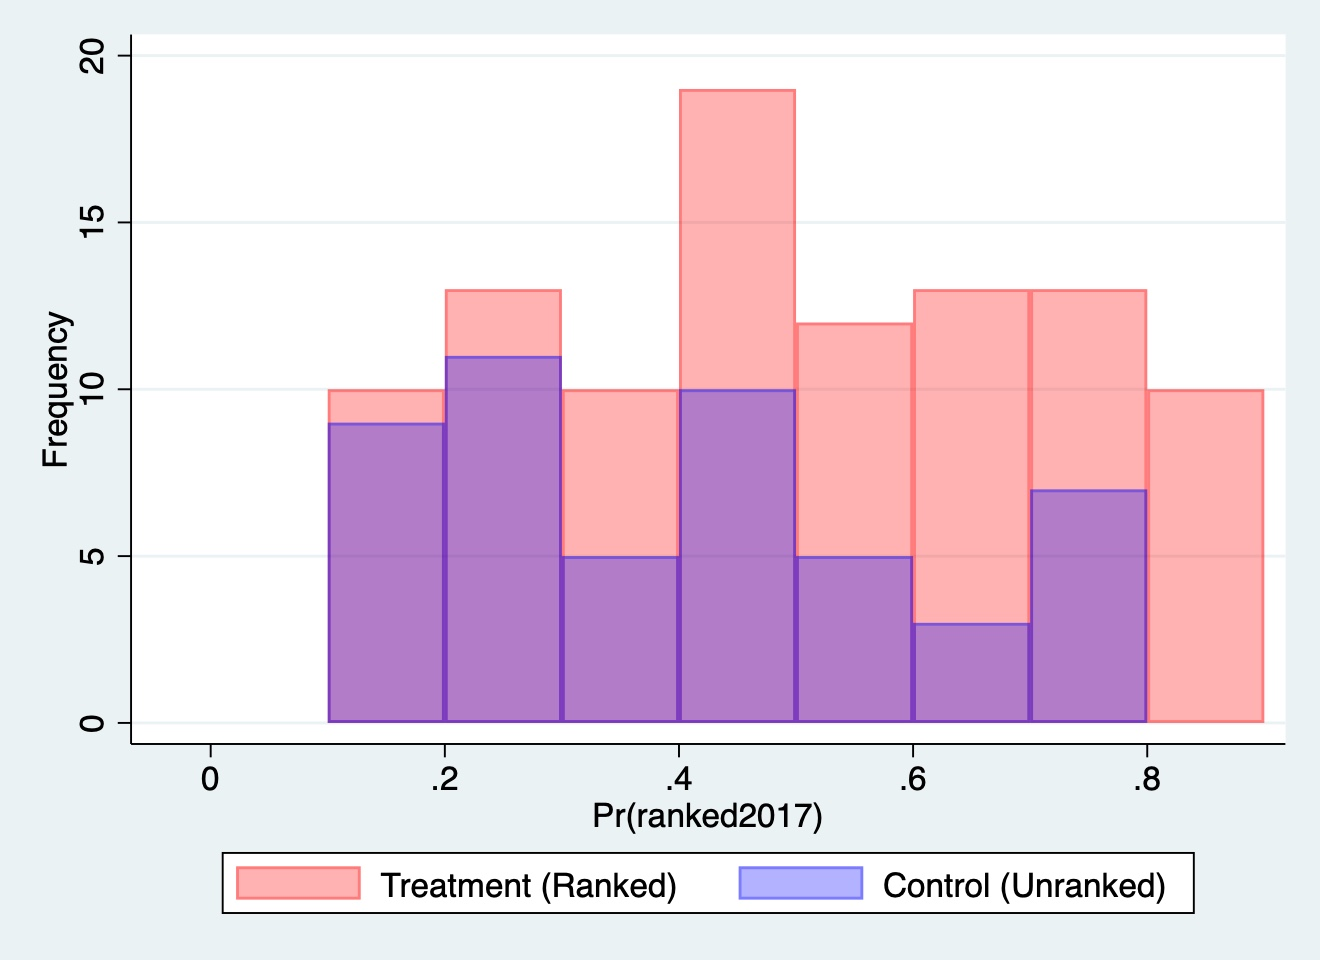
\includegraphics[width=90mm]{histogram.jpg}
    \center
    \begin{footnotesize}
    \textbf{Notes}: There is overlap between propensity scores of around 0.1 to 0.8. There are no treatment schools with propensity scores below 0.1 or above 0.9, and there are no control schools with propensity scores below 0.1 or above 0.8.
    \end{footnotesize}
\end{figure}
\newpage

\section{Propensity Score Model}
{
\def\sym#1{\ifmmode^{#1}\else\(^{#1}\)\fi}
\begin{longtable}{l*{1}{c}}
\hline\hline\endfirsthead\hline\endhead\hline\endfoot\endlastfoot
                    &\multicolumn{1}{c}{(1)}\\
                    &\multicolumn{1}{c}{Effect of Being Ranked on Alumni Donations}\\
\hline
Ranked 2017         &       500.6\sym{***}\\
                    &   (1806.97)         \\
[1em]
Academic Quality    &       99.05\sym{***}\\
                    &     (57.37)         \\
[1em]
Athletic Quality    &       52.45\sym{***}\\
                    &     (13.77)         \\
[1em]
Near Big Market     &      1001.7\sym{***}\\
                    &    (320.09)         \\
[1em]
block=1             &           0         \\
                    &         (.)         \\
[1em]
block=2             &       0.445         \\
                    &      (0.56)         \\
[1em]
block=3             &      -0.623         \\
                    &     (-0.66)         \\
[1em]
block=4             &       0.223         \\
                    &      (0.20)         \\
[1em]
block=5             &      -0.313         \\
                    &     (-0.25)         \\
[1em]
block=6             &      -0.478         \\
                    &     (-0.31)         \\
[1em]
block=7             &      -1.364         \\
                    &     (-0.67)         \\
[1em]
block=8             &      -1.523         \\
                    &     (-0.68)         \\
[1em]
block=9             &      -2.258         \\
                    &     (-0.87)         \\
[1em]
block=10            &      -2.049         \\
                    &     (-0.75)         \\
[1em]
block=11            &      -1.782         \\
                    &     (-0.62)         \\
[1em]
block=12            &      -1.330         \\
                    &     (-0.43)         \\
[1em]
block=13            &      -1.667         \\
                    &     (-0.51)         \\
[1em]
block=14            &      -2.084         \\
                    &     (-0.58)         \\
[1em]
block=15            &      -2.329         \\
                    &     (-0.62)         \\
[1em]
block=16            &      -3.192         \\
                    &     (-0.81)         \\
[1em]
block=17            &      -2.762         \\
                    &     (-0.66)         \\
[1em]
block=18            &      -2.837         \\
                    &     (-0.64)         \\
[1em]
block=19            &      -2.391         \\
                    &     (-0.51)         \\
[1em]
block=20            &      -2.522         \\
                    &     (-0.50)         \\
[1em]
block=21            &      -2.920         \\
                    &     (-0.56)         \\
[1em]
block=22            &      -3.671         \\
                    &     (-0.65)         \\
[1em]
block=23            &      -3.586         \\
                    &     (-0.61)         \\
[1em]
block=24            &      -4.066         \\
                    &     (-0.65)         \\
[1em]
block=25            &      -4.597         \\
                    &     (-0.67)         \\
[1em]
Constant            &       0.118         \\
                    &      (0.15)         \\
\hline
Observations        &         100         \\
\hline\hline
\multicolumn{2}{l}{\footnotesize \textit{t} statistics in parentheses}\\
\multicolumn{2}{l}{\footnotesize \sym{*} \(p<0.05\), \sym{**} \(p<0.01\), \sym{***} \(p<0.001\)}\\
\end{longtable}
}

\textbf{Notes}: This table contains a regression showing the effect of the predicted probability of being a top ranked basketball program on alumni donations. Here, we see that being ranked in 2017 is associated with a \$500,000 increase in alumni donations in 2018 relative to being unranked.


\end{document}
